\documentclass[a4paper,uplatex]{jsarticle}


% 数式
\usepackage{amsmath,amsfonts}
\usepackage{bm}
% 画像
\usepackage[dvipdfmx]{graphicx}
\usepackage{tikz}
\usepackage{gnuplot-lua-tikz}
% フォント
\usepackage[deluxe]{otf}

\usepackage{booktabs}

\numberwithin{equation}{section}
\numberwithin{figure}{section}
\numberwithin{table}{section}

\begin{document}

\title{PRML Chapter 1}
\author{}
\date{}
\maketitle

\section{例:多項式曲線フィッティング}
実数値の入力変数\(x\)を観測し、それを用いて実数値の目標変数\(t\)を予測する回帰問題を考える。ただし、ここでは関数\(\sin(2\pi x)\)にガウス分布に従う
ランダムノイズを加えて生成した人工データを用いる。

訓練集合として、\(N\)個の観測地\(x\)を並べた\(\bm{x} \equiv (x_1,\cdots,x_N)^T\)と、それぞれに対応する観測値\(t\)を並べた\(\bm{t} \equiv (t_1,\cdots,t_N)^T\)が与えられたとする。
図\ref{fig:toy data}は、\(N=10\)の場合の人工データの例である。

我々の目標は、この訓練集合を利用して、新たな入力変数\(\hat{x}\)に対して目標変数\(\hat{t}\)の値を予測することである。

\begin{figure}[htbp]
  \centering
  \begin{tikzpicture}[gnuplot]
%% generated with GNUPLOT 5.4p2 (Lua 5.4; terminal rev. Jun 2020, script rev. 114)
%% Wed Feb  7 22:18:47 2024
\path (0.000,0.000) rectangle (12.500,8.750);
\gpcolor{color=gp lt color border}
\gpsetlinetype{gp lt border}
\gpsetdashtype{gp dt solid}
\gpsetlinewidth{1.00}
\draw[gp path] (1.504,1.555)--(1.684,1.555);
\draw[gp path] (11.947,1.555)--(11.767,1.555);
\node[gp node right] at (1.320,1.555) {$-1$};
\draw[gp path] (1.504,2.980)--(1.684,2.980);
\draw[gp path] (11.947,2.980)--(11.767,2.980);
\node[gp node right] at (1.320,2.980) {$-0.5$};
\draw[gp path] (1.504,4.405)--(1.684,4.405);
\draw[gp path] (11.947,4.405)--(11.767,4.405);
\node[gp node right] at (1.320,4.405) {$0$};
\draw[gp path] (1.504,5.830)--(1.684,5.830);
\draw[gp path] (11.947,5.830)--(11.767,5.830);
\node[gp node right] at (1.320,5.830) {$0.5$};
\draw[gp path] (1.504,7.255)--(1.684,7.255);
\draw[gp path] (11.947,7.255)--(11.767,7.255);
\node[gp node right] at (1.320,7.255) {$1$};
\draw[gp path] (2.374,0.985)--(2.374,1.165);
\draw[gp path] (2.374,7.825)--(2.374,7.645);
\node[gp node center] at (2.374,0.677) {$0$};
\draw[gp path] (4.115,0.985)--(4.115,1.165);
\draw[gp path] (4.115,7.825)--(4.115,7.645);
\node[gp node center] at (4.115,0.677) {$0.2$};
\draw[gp path] (5.855,0.985)--(5.855,1.165);
\draw[gp path] (5.855,7.825)--(5.855,7.645);
\node[gp node center] at (5.855,0.677) {$0.4$};
\draw[gp path] (7.596,0.985)--(7.596,1.165);
\draw[gp path] (7.596,7.825)--(7.596,7.645);
\node[gp node center] at (7.596,0.677) {$0.6$};
\draw[gp path] (9.336,0.985)--(9.336,1.165);
\draw[gp path] (9.336,7.825)--(9.336,7.645);
\node[gp node center] at (9.336,0.677) {$0.8$};
\draw[gp path] (11.077,0.985)--(11.077,1.165);
\draw[gp path] (11.077,7.825)--(11.077,7.645);
\node[gp node center] at (11.077,0.677) {$1$};
\draw[gp path] (1.504,7.825)--(1.504,0.985)--(11.947,0.985)--(11.947,7.825)--cycle;
\node[gp node center,rotate=-270] at (0.292,4.405) {$t$};
\node[gp node center] at (6.725,0.215) {$x$};
\node[gp node right] at (10.479,7.491) {$\sin(2\pi x)$};
\gpcolor{rgb color={0.000,1.000,0.000}}
\draw[gp path] (10.663,7.491)--(11.579,7.491);
\draw[gp path] (1.504,2.730)--(1.609,2.910)--(1.715,3.099)--(1.820,3.296)--(1.926,3.499)%
  --(2.031,3.707)--(2.137,3.919)--(2.242,4.134)--(2.348,4.351)--(2.453,4.568)--(2.559,4.784)%
  --(2.664,4.998)--(2.770,5.208)--(2.875,5.414)--(2.981,5.614)--(3.086,5.806)--(3.192,5.991)%
  --(3.297,6.167)--(3.403,6.332)--(3.508,6.486)--(3.614,6.628)--(3.719,6.758)--(3.825,6.873)%
  --(3.930,6.974)--(4.036,7.061)--(4.141,7.132)--(4.247,7.187)--(4.352,7.226)--(4.458,7.249)%
  --(4.563,7.255)--(4.669,7.245)--(4.774,7.218)--(4.880,7.175)--(4.985,7.116)--(5.090,7.041)%
  --(5.196,6.950)--(5.301,6.846)--(5.407,6.727)--(5.512,6.594)--(5.618,6.449)--(5.723,6.292)%
  --(5.829,6.124)--(5.934,5.946)--(6.040,5.759)--(6.145,5.564)--(6.251,5.363)--(6.356,5.156)%
  --(6.462,4.944)--(6.567,4.730)--(6.673,4.514)--(6.778,4.296)--(6.884,4.080)--(6.989,3.866)%
  --(7.095,3.654)--(7.200,3.447)--(7.306,3.246)--(7.411,3.051)--(7.517,2.864)--(7.622,2.686)%
  --(7.728,2.518)--(7.833,2.361)--(7.939,2.216)--(8.044,2.083)--(8.150,1.964)--(8.255,1.860)%
  --(8.361,1.769)--(8.466,1.694)--(8.571,1.635)--(8.677,1.592)--(8.782,1.565)--(8.888,1.555)%
  --(8.993,1.561)--(9.099,1.584)--(9.204,1.623)--(9.310,1.678)--(9.415,1.749)--(9.521,1.836)%
  --(9.626,1.937)--(9.732,2.052)--(9.837,2.182)--(9.943,2.324)--(10.048,2.478)--(10.154,2.643)%
  --(10.259,2.819)--(10.365,3.004)--(10.470,3.196)--(10.576,3.396)--(10.681,3.602)--(10.787,3.812)%
  --(10.892,4.026)--(10.998,4.242)--(11.103,4.459)--(11.209,4.676)--(11.314,4.891)--(11.420,5.103)%
  --(11.525,5.311)--(11.631,5.514)--(11.736,5.711)--(11.842,5.900)--(11.947,6.080);
\gpcolor{color=gp lt color border}
\node[gp node right] at (10.479,7.183) {$\sin(2\pi x) + noise$};
\gpcolor{rgb color={0.000,0.000,1.000}}
\gpsetpointsize{4.00}
\gp3point{gp mark 7}{}{(2.374,4.091)}
\gp3point{gp mark 7}{}{(3.332,6.457)}
\gp3point{gp mark 7}{}{(4.289,7.056)}
\gp3point{gp mark 7}{}{(5.246,6.229)}
\gp3point{gp mark 7}{}{(6.203,5.004)}
\gp3point{gp mark 7}{}{(7.248,3.294)}
\gp3point{gp mark 7}{}{(8.205,1.355)}
\gp3point{gp mark 7}{}{(9.162,1.099)}
\gp3point{gp mark 7}{}{(10.119,3.208)}
\gp3point{gp mark 7}{}{(11.077,4.890)}
\gp3point{gp mark 7}{}{(11.121,7.183)}
\gpcolor{color=gp lt color border}
\draw[gp path] (1.504,7.825)--(1.504,0.985)--(11.947,0.985)--(11.947,7.825)--cycle;
\node[gp node center] at (6.725,8.287) {Toy Dataset};
%% coordinates of the plot area
\gpdefrectangularnode{gp plot 1}{\pgfpoint{1.504cm}{0.985cm}}{\pgfpoint{11.947cm}{7.825cm}}
\end{tikzpicture}

  \caption{\(N=10\)個の訓練データの例}
  \label{fig:toy data}
\end{figure}

ここでは、以下のような多項式を用いてデータへのフィッティングを行うことにする。
\begin{equation}
  y(x,\bm{w}) = w_0 + w_1 x + w_2 x^2 + \cdots + w_M x^M = \sum_{j=0}^{M} w_j x^j
\end{equation}
ただし、\(M\)は多項式の\textbf{次数(order)}で、\(x^j\)は\(x\)の\(j\)乗を表す。多項式の係数\(w_0,\cdots,w_M\)をまとめて\(\bm{w}\)と書くことにする。
多項式\(y(x,\bm{w})\)は、\(x\)の非線形関数であるが、係数\(\bm{w}\)の線形関数であることに注意する。このような、未知パラメータに対して線形な関数は\textbf{線形モデル}と呼ばれる。

訓練データに多項式をあてはめることで係数の値を求める。これは、\(\bm{w}\)を任意に固定したときの関数\(y(x,\bm{w})\)と
訓練集合のデータ点との間のずれを測る\textbf{誤差関数(error function)}の最小化で達成できる。ここでは、誤差関数として単純で広く用いられている\textbf{二乗和誤差(sum-of-squares error)}を用いる。
式で書けば、
\begin{equation}
  E(\bm{w}) = \frac{1}{2} \sum_{n=1}^{N} \{y(x_n,\bm{w}) - t_n\}^2
\end{equation}
となる。ただし、後で便利なように係数\(1/2\)をかけている。

このように、\(E(\bm{w})\)をできるだけ小さくするような\(\bm{w}\)を選ぶことで曲線当てはめ問題を解くことができる。では、誤差関数を最小にする解\(\bm{w^*}=\{w_i\}\)を求める。
誤差関数を最小にする解をもとめるには、\(E(\bm{w})\)を\(w_i\)について微分し、その微分がゼロになるような\(w_i\)を求めればよい。
つまり、
\begin{equation}
  \frac{\delta E}{\delta w_i} = 0
\end{equation}
を求める。
はじめに、\(E(\bm{w})\)を\(w_i\)について微分する。
\begin{align*}
  \frac{\delta E}{\delta w_i} &= \frac{1}{2}\sum_{n=1}^{N}\left\{2\left(\sum_{j=0}^{M}w_j x_n^j-t_n\right)-x_n^i\right\} \\
                              &= \sum_{n=1}^{N}\left(x_n^i\sum_{j=0}^{M}w_j x_n^j\right) - \sum_{n=1}^{N}t_n x_n^i \\
\end{align*}
ここで、\(\frac{\delta E}{\delta w_i} = 0\)を求めるので、
\begin{equation}
  \sum_{n=1}^{N}\left(x_n^i\sum_{j=0}^{M}w_j x_n^j\right) = \sum_{n=1}^{N}t_n x_n^i
\end{equation}

左辺を変形すると、
\begin{align*}
  (左辺) &= \sum_{n=1}^{N}\left\{x_n^i\left(w_0 x_n^0+w_1x_n^1+\cdots+w_Mx_n^M\right)\right\} \\
         &= \sum_{n=1}^{N}\left\{w_0x_n^{i+0}+w_1x_n^{i+1}+\cdots+w_Mx_n^{i+M}\right\} \\
         &= \sum_{n=1}^{N}\sum_{j=0}^{M}\left(w_jx_n^{i+j}\right) \\
         &= \sum_{j=0}^{M}\left\{\sum_{n=1}^{N}(x_n)^{i+j}\right\}w_j \\
\end{align*}
また、
\begin{equation}
  A_{ij} = \sum_{n=1}^{N}(x_n)^{i+j}, T_i = \sum_{n=1}^{N}t_n(x_n)^i
\end{equation}
とおくと、
\begin{equation}
  \sum_{j=0}^{M}A_{ij}w_j = T_i
\end{equation}
となる。これは線形方程式であり、これを解くことで、誤差関数を最小にする解\(\bm{w^*}\)を求めることができる。

\begin{figure}[htbp]
  \centering
  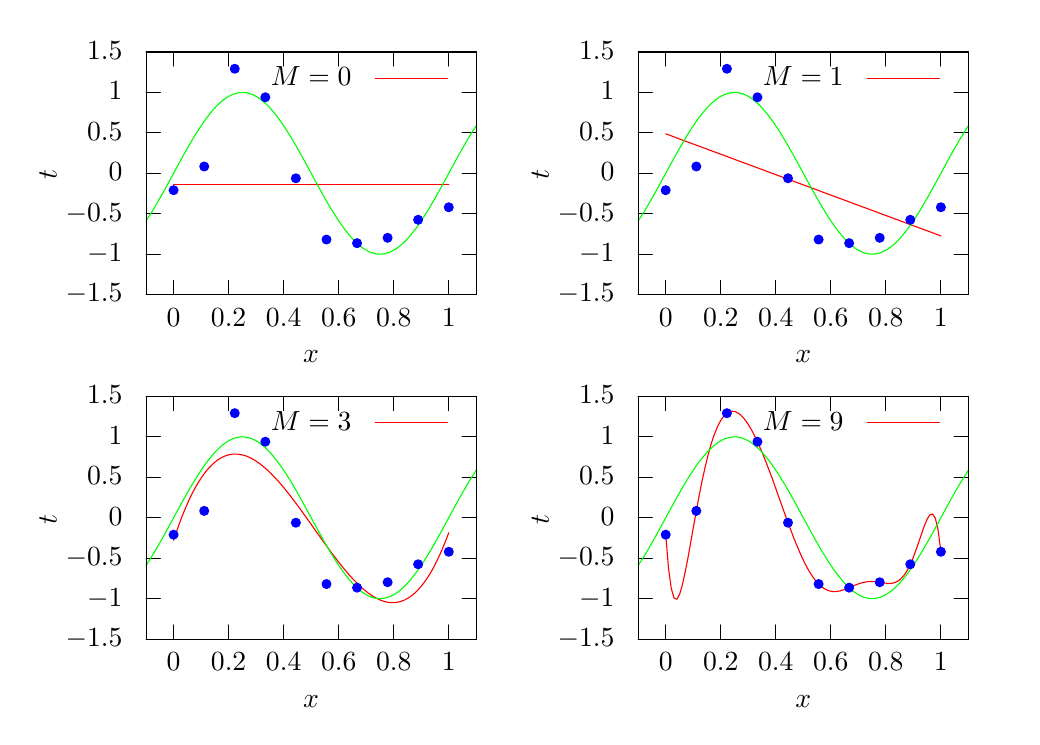
\begin{tikzpicture}[gnuplot]
%% generated with GNUPLOT 5.4p2 (Lua 5.4; terminal rev. Jun 2020, script rev. 114)
%% Tue Feb 27 20:55:19 2024
\path (0.000,0.000) rectangle (12.500,8.750);
\gpcolor{color=gp lt color border}
\gpsetlinetype{gp lt border}
\gpsetdashtype{gp dt solid}
\gpsetlinewidth{1.00}
\draw[gp path] (1.504,5.360)--(1.684,5.360);
\draw[gp path] (5.697,5.360)--(5.517,5.360);
\node[gp node right] at (1.320,5.360) {$-1.5$};
\draw[gp path] (1.504,5.874)--(1.684,5.874);
\draw[gp path] (5.697,5.874)--(5.517,5.874);
\node[gp node right] at (1.320,5.874) {$-1$};
\draw[gp path] (1.504,6.387)--(1.684,6.387);
\draw[gp path] (5.697,6.387)--(5.517,6.387);
\node[gp node right] at (1.320,6.387) {$-0.5$};
\draw[gp path] (1.504,6.901)--(1.684,6.901);
\draw[gp path] (5.697,6.901)--(5.517,6.901);
\node[gp node right] at (1.320,6.901) {$0$};
\draw[gp path] (1.504,7.414)--(1.684,7.414);
\draw[gp path] (5.697,7.414)--(5.517,7.414);
\node[gp node right] at (1.320,7.414) {$0.5$};
\draw[gp path] (1.504,7.928)--(1.684,7.928);
\draw[gp path] (5.697,7.928)--(5.517,7.928);
\node[gp node right] at (1.320,7.928) {$1$};
\draw[gp path] (1.504,8.441)--(1.684,8.441);
\draw[gp path] (5.697,8.441)--(5.517,8.441);
\node[gp node right] at (1.320,8.441) {$1.5$};
\draw[gp path] (1.853,5.360)--(1.853,5.540);
\draw[gp path] (1.853,8.441)--(1.853,8.261);
\node[gp node center] at (1.853,5.052) {$0$};
\draw[gp path] (2.552,5.360)--(2.552,5.540);
\draw[gp path] (2.552,8.441)--(2.552,8.261);
\node[gp node center] at (2.552,5.052) {$0.2$};
\draw[gp path] (3.251,5.360)--(3.251,5.540);
\draw[gp path] (3.251,8.441)--(3.251,8.261);
\node[gp node center] at (3.251,5.052) {$0.4$};
\draw[gp path] (3.950,5.360)--(3.950,5.540);
\draw[gp path] (3.950,8.441)--(3.950,8.261);
\node[gp node center] at (3.950,5.052) {$0.6$};
\draw[gp path] (4.649,5.360)--(4.649,5.540);
\draw[gp path] (4.649,8.441)--(4.649,8.261);
\node[gp node center] at (4.649,5.052) {$0.8$};
\draw[gp path] (5.348,5.360)--(5.348,5.540);
\draw[gp path] (5.348,8.441)--(5.348,8.261);
\node[gp node center] at (5.348,5.052) {$1$};
\draw[gp path] (1.504,8.441)--(1.504,5.360)--(5.697,5.360)--(5.697,8.441)--cycle;
\node[gp node center,rotate=-270] at (0.292,6.900) {$t$};
\node[gp node center] at (3.600,4.590) {$x$};
\node[gp node right] at (4.229,8.107) {$M=0$};
\gpcolor{rgb color={1.000,0.000,0.000}}
\draw[gp path] (4.413,8.107)--(5.329,8.107);
\draw[gp path] (1.853,6.754)--(1.889,6.754)--(1.924,6.754)--(1.959,6.754)--(1.995,6.754)%
  --(2.030,6.754)--(2.065,6.754)--(2.100,6.754)--(2.136,6.754)--(2.171,6.754)--(2.206,6.754)%
  --(2.242,6.754)--(2.277,6.754)--(2.312,6.754)--(2.348,6.754)--(2.383,6.754)--(2.418,6.754)%
  --(2.453,6.754)--(2.489,6.754)--(2.524,6.754)--(2.559,6.754)--(2.595,6.754)--(2.630,6.754)%
  --(2.665,6.754)--(2.700,6.754)--(2.736,6.754)--(2.771,6.754)--(2.806,6.754)--(2.842,6.754)%
  --(2.877,6.754)--(2.912,6.754)--(2.948,6.754)--(2.983,6.754)--(3.018,6.754)--(3.053,6.754)%
  --(3.089,6.754)--(3.124,6.754)--(3.159,6.754)--(3.195,6.754)--(3.230,6.754)--(3.265,6.754)%
  --(3.300,6.754)--(3.336,6.754)--(3.371,6.754)--(3.406,6.754)--(3.442,6.754)--(3.477,6.754)%
  --(3.512,6.754)--(3.548,6.754)--(3.583,6.754)--(3.618,6.754)--(3.653,6.754)--(3.689,6.754)%
  --(3.724,6.754)--(3.759,6.754)--(3.795,6.754)--(3.830,6.754)--(3.865,6.754)--(3.901,6.754)%
  --(3.936,6.754)--(3.971,6.754)--(4.006,6.754)--(4.042,6.754)--(4.077,6.754)--(4.112,6.754)%
  --(4.148,6.754)--(4.183,6.754)--(4.218,6.754)--(4.253,6.754)--(4.289,6.754)--(4.324,6.754)%
  --(4.359,6.754)--(4.395,6.754)--(4.430,6.754)--(4.465,6.754)--(4.501,6.754)--(4.536,6.754)%
  --(4.571,6.754)--(4.606,6.754)--(4.642,6.754)--(4.677,6.754)--(4.712,6.754)--(4.748,6.754)%
  --(4.783,6.754)--(4.818,6.754)--(4.853,6.754)--(4.889,6.754)--(4.924,6.754)--(4.959,6.754)%
  --(4.995,6.754)--(5.030,6.754)--(5.065,6.754)--(5.101,6.754)--(5.136,6.754)--(5.171,6.754)%
  --(5.206,6.754)--(5.242,6.754)--(5.277,6.754)--(5.312,6.754)--(5.348,6.754);
\gpcolor{rgb color={0.000,1.000,0.000}}
\draw[gp path] (1.504,6.297)--(1.546,6.362)--(1.589,6.430)--(1.631,6.501)--(1.673,6.574)%
  --(1.716,6.649)--(1.758,6.725)--(1.800,6.803)--(1.843,6.881)--(1.885,6.959)--(1.928,7.037)%
  --(1.970,7.114)--(2.012,7.190)--(2.055,7.264)--(2.097,7.336)--(2.139,7.406)--(2.182,7.472)%
  --(2.224,7.535)--(2.266,7.595)--(2.309,7.650)--(2.351,7.702)--(2.393,7.748)--(2.436,7.790)%
  --(2.478,7.826)--(2.520,7.858)--(2.563,7.883)--(2.605,7.903)--(2.648,7.917)--(2.690,7.925)%
  --(2.732,7.927)--(2.775,7.924)--(2.817,7.914)--(2.859,7.899)--(2.902,7.877)--(2.944,7.850)%
  --(2.986,7.818)--(3.029,7.780)--(3.071,7.737)--(3.113,7.689)--(3.156,7.637)--(3.198,7.580)%
  --(3.240,7.520)--(3.283,7.456)--(3.325,7.388)--(3.368,7.318)--(3.410,7.246)--(3.452,7.171)%
  --(3.495,7.095)--(3.537,7.018)--(3.579,6.940)--(3.622,6.861)--(3.664,6.783)--(3.706,6.706)%
  --(3.749,6.630)--(3.791,6.555)--(3.833,6.483)--(3.876,6.413)--(3.918,6.345)--(3.961,6.281)%
  --(4.003,6.221)--(4.045,6.164)--(4.088,6.112)--(4.130,6.064)--(4.172,6.021)--(4.215,5.983)%
  --(4.257,5.951)--(4.299,5.924)--(4.342,5.902)--(4.384,5.887)--(4.426,5.877)--(4.469,5.874)%
  --(4.511,5.876)--(4.553,5.884)--(4.596,5.898)--(4.638,5.918)--(4.681,5.943)--(4.723,5.975)%
  --(4.765,6.011)--(4.808,6.053)--(4.850,6.099)--(4.892,6.151)--(4.935,6.206)--(4.977,6.266)%
  --(5.019,6.329)--(5.062,6.395)--(5.104,6.465)--(5.146,6.537)--(5.189,6.611)--(5.231,6.687)%
  --(5.273,6.764)--(5.316,6.842)--(5.358,6.920)--(5.401,6.998)--(5.443,7.076)--(5.485,7.152)%
  --(5.528,7.227)--(5.570,7.300)--(5.612,7.371)--(5.655,7.439)--(5.697,7.504);
\gpcolor{rgb color={0.000,0.000,1.000}}
\gpsetpointsize{4.00}
\gp3point{gp mark 7}{}{(1.853,6.686)}
\gp3point{gp mark 7}{}{(2.242,6.987)}
\gp3point{gp mark 7}{}{(2.630,8.228)}
\gp3point{gp mark 7}{}{(3.018,7.866)}
\gp3point{gp mark 7}{}{(3.406,6.837)}
\gp3point{gp mark 7}{}{(3.795,6.059)}
\gp3point{gp mark 7}{}{(4.183,6.013)}
\gp3point{gp mark 7}{}{(4.571,6.081)}
\gp3point{gp mark 7}{}{(4.959,6.310)}
\gp3point{gp mark 7}{}{(5.348,6.469)}
\gpcolor{color=gp lt color border}
\draw[gp path] (1.504,8.441)--(1.504,5.360)--(5.697,5.360)--(5.697,8.441)--cycle;
%% coordinates of the plot area
\gpdefrectangularnode{gp plot 1}{\pgfpoint{1.504cm}{5.360cm}}{\pgfpoint{5.697cm}{8.441cm}}
\draw[gp path] (7.754,5.360)--(7.934,5.360);
\draw[gp path] (11.947,5.360)--(11.767,5.360);
\node[gp node right] at (7.570,5.360) {$-1.5$};
\draw[gp path] (7.754,5.874)--(7.934,5.874);
\draw[gp path] (11.947,5.874)--(11.767,5.874);
\node[gp node right] at (7.570,5.874) {$-1$};
\draw[gp path] (7.754,6.387)--(7.934,6.387);
\draw[gp path] (11.947,6.387)--(11.767,6.387);
\node[gp node right] at (7.570,6.387) {$-0.5$};
\draw[gp path] (7.754,6.901)--(7.934,6.901);
\draw[gp path] (11.947,6.901)--(11.767,6.901);
\node[gp node right] at (7.570,6.901) {$0$};
\draw[gp path] (7.754,7.414)--(7.934,7.414);
\draw[gp path] (11.947,7.414)--(11.767,7.414);
\node[gp node right] at (7.570,7.414) {$0.5$};
\draw[gp path] (7.754,7.928)--(7.934,7.928);
\draw[gp path] (11.947,7.928)--(11.767,7.928);
\node[gp node right] at (7.570,7.928) {$1$};
\draw[gp path] (7.754,8.441)--(7.934,8.441);
\draw[gp path] (11.947,8.441)--(11.767,8.441);
\node[gp node right] at (7.570,8.441) {$1.5$};
\draw[gp path] (8.103,5.360)--(8.103,5.540);
\draw[gp path] (8.103,8.441)--(8.103,8.261);
\node[gp node center] at (8.103,5.052) {$0$};
\draw[gp path] (8.802,5.360)--(8.802,5.540);
\draw[gp path] (8.802,8.441)--(8.802,8.261);
\node[gp node center] at (8.802,5.052) {$0.2$};
\draw[gp path] (9.501,5.360)--(9.501,5.540);
\draw[gp path] (9.501,8.441)--(9.501,8.261);
\node[gp node center] at (9.501,5.052) {$0.4$};
\draw[gp path] (10.200,5.360)--(10.200,5.540);
\draw[gp path] (10.200,8.441)--(10.200,8.261);
\node[gp node center] at (10.200,5.052) {$0.6$};
\draw[gp path] (10.899,5.360)--(10.899,5.540);
\draw[gp path] (10.899,8.441)--(10.899,8.261);
\node[gp node center] at (10.899,5.052) {$0.8$};
\draw[gp path] (11.598,5.360)--(11.598,5.540);
\draw[gp path] (11.598,8.441)--(11.598,8.261);
\node[gp node center] at (11.598,5.052) {$1$};
\draw[gp path] (7.754,8.441)--(7.754,5.360)--(11.947,5.360)--(11.947,8.441)--cycle;
\node[gp node center,rotate=-270] at (6.542,6.900) {$t$};
\node[gp node center] at (9.850,4.590) {$x$};
\node[gp node right] at (10.479,8.107) {$M=1$};
\gpcolor{rgb color={1.000,0.000,0.000}}
\draw[gp path] (10.663,8.107)--(11.579,8.107);
\draw[gp path] (8.103,7.402)--(8.139,7.389)--(8.174,7.376)--(8.209,7.363)--(8.245,7.349)%
  --(8.280,7.336)--(8.315,7.323)--(8.350,7.310)--(8.386,7.297)--(8.421,7.284)--(8.456,7.271)%
  --(8.492,7.258)--(8.527,7.245)--(8.562,7.232)--(8.598,7.219)--(8.633,7.205)--(8.668,7.192)%
  --(8.703,7.179)--(8.739,7.166)--(8.774,7.153)--(8.809,7.140)--(8.845,7.127)--(8.880,7.114)%
  --(8.915,7.101)--(8.950,7.088)--(8.986,7.074)--(9.021,7.061)--(9.056,7.048)--(9.092,7.035)%
  --(9.127,7.022)--(9.162,7.009)--(9.198,6.996)--(9.233,6.983)--(9.268,6.970)--(9.303,6.957)%
  --(9.339,6.944)--(9.374,6.930)--(9.409,6.917)--(9.445,6.904)--(9.480,6.891)--(9.515,6.878)%
  --(9.550,6.865)--(9.586,6.852)--(9.621,6.839)--(9.656,6.826)--(9.692,6.813)--(9.727,6.799)%
  --(9.762,6.786)--(9.798,6.773)--(9.833,6.760)--(9.868,6.747)--(9.903,6.734)--(9.939,6.721)%
  --(9.974,6.708)--(10.009,6.695)--(10.045,6.682)--(10.080,6.668)--(10.115,6.655)--(10.151,6.642)%
  --(10.186,6.629)--(10.221,6.616)--(10.256,6.603)--(10.292,6.590)--(10.327,6.577)--(10.362,6.564)%
  --(10.398,6.551)--(10.433,6.538)--(10.468,6.524)--(10.503,6.511)--(10.539,6.498)--(10.574,6.485)%
  --(10.609,6.472)--(10.645,6.459)--(10.680,6.446)--(10.715,6.433)--(10.751,6.420)--(10.786,6.407)%
  --(10.821,6.393)--(10.856,6.380)--(10.892,6.367)--(10.927,6.354)--(10.962,6.341)--(10.998,6.328)%
  --(11.033,6.315)--(11.068,6.302)--(11.103,6.289)--(11.139,6.276)--(11.174,6.262)--(11.209,6.249)%
  --(11.245,6.236)--(11.280,6.223)--(11.315,6.210)--(11.351,6.197)--(11.386,6.184)--(11.421,6.171)%
  --(11.456,6.158)--(11.492,6.145)--(11.527,6.132)--(11.562,6.118)--(11.598,6.105);
\gpcolor{rgb color={0.000,1.000,0.000}}
\draw[gp path] (7.754,6.297)--(7.796,6.362)--(7.839,6.430)--(7.881,6.501)--(7.923,6.574)%
  --(7.966,6.649)--(8.008,6.725)--(8.050,6.803)--(8.093,6.881)--(8.135,6.959)--(8.178,7.037)%
  --(8.220,7.114)--(8.262,7.190)--(8.305,7.264)--(8.347,7.336)--(8.389,7.406)--(8.432,7.472)%
  --(8.474,7.535)--(8.516,7.595)--(8.559,7.650)--(8.601,7.702)--(8.643,7.748)--(8.686,7.790)%
  --(8.728,7.826)--(8.770,7.858)--(8.813,7.883)--(8.855,7.903)--(8.898,7.917)--(8.940,7.925)%
  --(8.982,7.927)--(9.025,7.924)--(9.067,7.914)--(9.109,7.899)--(9.152,7.877)--(9.194,7.850)%
  --(9.236,7.818)--(9.279,7.780)--(9.321,7.737)--(9.363,7.689)--(9.406,7.637)--(9.448,7.580)%
  --(9.490,7.520)--(9.533,7.456)--(9.575,7.388)--(9.618,7.318)--(9.660,7.246)--(9.702,7.171)%
  --(9.745,7.095)--(9.787,7.018)--(9.829,6.940)--(9.872,6.861)--(9.914,6.783)--(9.956,6.706)%
  --(9.999,6.630)--(10.041,6.555)--(10.083,6.483)--(10.126,6.413)--(10.168,6.345)--(10.211,6.281)%
  --(10.253,6.221)--(10.295,6.164)--(10.338,6.112)--(10.380,6.064)--(10.422,6.021)--(10.465,5.983)%
  --(10.507,5.951)--(10.549,5.924)--(10.592,5.902)--(10.634,5.887)--(10.676,5.877)--(10.719,5.874)%
  --(10.761,5.876)--(10.803,5.884)--(10.846,5.898)--(10.888,5.918)--(10.931,5.943)--(10.973,5.975)%
  --(11.015,6.011)--(11.058,6.053)--(11.100,6.099)--(11.142,6.151)--(11.185,6.206)--(11.227,6.266)%
  --(11.269,6.329)--(11.312,6.395)--(11.354,6.465)--(11.396,6.537)--(11.439,6.611)--(11.481,6.687)%
  --(11.523,6.764)--(11.566,6.842)--(11.608,6.920)--(11.651,6.998)--(11.693,7.076)--(11.735,7.152)%
  --(11.778,7.227)--(11.820,7.300)--(11.862,7.371)--(11.905,7.439)--(11.947,7.504);
\gpcolor{rgb color={0.000,0.000,1.000}}
\gp3point{gp mark 7}{}{(8.103,6.686)}
\gp3point{gp mark 7}{}{(8.492,6.987)}
\gp3point{gp mark 7}{}{(8.880,8.228)}
\gp3point{gp mark 7}{}{(9.268,7.866)}
\gp3point{gp mark 7}{}{(9.656,6.837)}
\gp3point{gp mark 7}{}{(10.045,6.059)}
\gp3point{gp mark 7}{}{(10.433,6.013)}
\gp3point{gp mark 7}{}{(10.821,6.081)}
\gp3point{gp mark 7}{}{(11.209,6.310)}
\gp3point{gp mark 7}{}{(11.598,6.469)}
\gpcolor{color=gp lt color border}
\draw[gp path] (7.754,8.441)--(7.754,5.360)--(11.947,5.360)--(11.947,8.441)--cycle;
%% coordinates of the plot area
\gpdefrectangularnode{gp plot 2}{\pgfpoint{7.754cm}{5.360cm}}{\pgfpoint{11.947cm}{8.441cm}}
\draw[gp path] (1.504,0.985)--(1.684,0.985);
\draw[gp path] (5.697,0.985)--(5.517,0.985);
\node[gp node right] at (1.320,0.985) {$-1.5$};
\draw[gp path] (1.504,1.499)--(1.684,1.499);
\draw[gp path] (5.697,1.499)--(5.517,1.499);
\node[gp node right] at (1.320,1.499) {$-1$};
\draw[gp path] (1.504,2.012)--(1.684,2.012);
\draw[gp path] (5.697,2.012)--(5.517,2.012);
\node[gp node right] at (1.320,2.012) {$-0.5$};
\draw[gp path] (1.504,2.526)--(1.684,2.526);
\draw[gp path] (5.697,2.526)--(5.517,2.526);
\node[gp node right] at (1.320,2.526) {$0$};
\draw[gp path] (1.504,3.040)--(1.684,3.040);
\draw[gp path] (5.697,3.040)--(5.517,3.040);
\node[gp node right] at (1.320,3.040) {$0.5$};
\draw[gp path] (1.504,3.553)--(1.684,3.553);
\draw[gp path] (5.697,3.553)--(5.517,3.553);
\node[gp node right] at (1.320,3.553) {$1$};
\draw[gp path] (1.504,4.067)--(1.684,4.067);
\draw[gp path] (5.697,4.067)--(5.517,4.067);
\node[gp node right] at (1.320,4.067) {$1.5$};
\draw[gp path] (1.853,0.985)--(1.853,1.165);
\draw[gp path] (1.853,4.067)--(1.853,3.887);
\node[gp node center] at (1.853,0.677) {$0$};
\draw[gp path] (2.552,0.985)--(2.552,1.165);
\draw[gp path] (2.552,4.067)--(2.552,3.887);
\node[gp node center] at (2.552,0.677) {$0.2$};
\draw[gp path] (3.251,0.985)--(3.251,1.165);
\draw[gp path] (3.251,4.067)--(3.251,3.887);
\node[gp node center] at (3.251,0.677) {$0.4$};
\draw[gp path] (3.950,0.985)--(3.950,1.165);
\draw[gp path] (3.950,4.067)--(3.950,3.887);
\node[gp node center] at (3.950,0.677) {$0.6$};
\draw[gp path] (4.649,0.985)--(4.649,1.165);
\draw[gp path] (4.649,4.067)--(4.649,3.887);
\node[gp node center] at (4.649,0.677) {$0.8$};
\draw[gp path] (5.348,0.985)--(5.348,1.165);
\draw[gp path] (5.348,4.067)--(5.348,3.887);
\node[gp node center] at (5.348,0.677) {$1$};
\draw[gp path] (1.504,4.067)--(1.504,0.985)--(5.697,0.985)--(5.697,4.067)--cycle;
\node[gp node center,rotate=-270] at (0.292,2.526) {$t$};
\node[gp node center] at (3.600,0.215) {$x$};
\node[gp node right] at (4.229,3.733) {$M=3$};
\gpcolor{rgb color={1.000,0.000,0.000}}
\draw[gp path] (4.413,3.733)--(5.329,3.733);
\draw[gp path] (1.853,2.240)--(1.889,2.345)--(1.924,2.445)--(1.959,2.539)--(1.995,2.626)%
  --(2.030,2.708)--(2.065,2.785)--(2.100,2.855)--(2.136,2.921)--(2.171,2.981)--(2.206,3.035)%
  --(2.242,3.085)--(2.277,3.130)--(2.312,3.170)--(2.348,3.205)--(2.383,3.236)--(2.418,3.263)%
  --(2.453,3.285)--(2.489,3.303)--(2.524,3.317)--(2.559,3.326)--(2.595,3.333)--(2.630,3.335)%
  --(2.665,3.334)--(2.700,3.329)--(2.736,3.322)--(2.771,3.311)--(2.806,3.297)--(2.842,3.280)%
  --(2.877,3.260)--(2.912,3.237)--(2.948,3.212)--(2.983,3.185)--(3.018,3.155)--(3.053,3.123)%
  --(3.089,3.089)--(3.124,3.053)--(3.159,3.015)--(3.195,2.976)--(3.230,2.935)--(3.265,2.893)%
  --(3.300,2.849)--(3.336,2.804)--(3.371,2.758)--(3.406,2.711)--(3.442,2.663)--(3.477,2.615)%
  --(3.512,2.566)--(3.548,2.516)--(3.583,2.467)--(3.618,2.417)--(3.653,2.367)--(3.689,2.317)%
  --(3.724,2.267)--(3.759,2.218)--(3.795,2.169)--(3.830,2.120)--(3.865,2.073)--(3.901,2.026)%
  --(3.936,1.980)--(3.971,1.935)--(4.006,1.891)--(4.042,1.849)--(4.077,1.808)--(4.112,1.768)%
  --(4.148,1.730)--(4.183,1.694)--(4.218,1.660)--(4.253,1.628)--(4.289,1.599)--(4.324,1.571)%
  --(4.359,1.546)--(4.395,1.523)--(4.430,1.504)--(4.465,1.487)--(4.501,1.472)--(4.536,1.461)%
  --(4.571,1.453)--(4.606,1.449)--(4.642,1.448)--(4.677,1.450)--(4.712,1.456)--(4.748,1.466)%
  --(4.783,1.480)--(4.818,1.498)--(4.853,1.520)--(4.889,1.546)--(4.924,1.577)--(4.959,1.612)%
  --(4.995,1.652)--(5.030,1.697)--(5.065,1.746)--(5.101,1.801)--(5.136,1.861)--(5.171,1.926)%
  --(5.206,1.997)--(5.242,2.073)--(5.277,2.155)--(5.312,2.242)--(5.348,2.336);
\gpcolor{rgb color={0.000,1.000,0.000}}
\draw[gp path] (1.504,1.922)--(1.546,1.987)--(1.589,2.055)--(1.631,2.126)--(1.673,2.199)%
  --(1.716,2.274)--(1.758,2.351)--(1.800,2.428)--(1.843,2.506)--(1.885,2.585)--(1.928,2.663)%
  --(1.970,2.740)--(2.012,2.815)--(2.055,2.890)--(2.097,2.962)--(2.139,3.031)--(2.182,3.098)%
  --(2.224,3.161)--(2.266,3.221)--(2.309,3.276)--(2.351,3.327)--(2.393,3.374)--(2.436,3.416)%
  --(2.478,3.452)--(2.520,3.483)--(2.563,3.509)--(2.605,3.529)--(2.648,3.543)--(2.690,3.551)%
  --(2.732,3.553)--(2.775,3.550)--(2.817,3.540)--(2.859,3.524)--(2.902,3.503)--(2.944,3.476)%
  --(2.986,3.444)--(3.029,3.406)--(3.071,3.363)--(3.113,3.315)--(3.156,3.263)--(3.198,3.206)%
  --(3.240,3.146)--(3.283,3.081)--(3.325,3.014)--(3.368,2.944)--(3.410,2.871)--(3.452,2.797)%
  --(3.495,2.720)--(3.537,2.643)--(3.579,2.565)--(3.622,2.487)--(3.664,2.409)--(3.706,2.332)%
  --(3.749,2.255)--(3.791,2.181)--(3.833,2.108)--(3.876,2.038)--(3.918,1.971)--(3.961,1.906)%
  --(4.003,1.846)--(4.045,1.789)--(4.088,1.737)--(4.130,1.689)--(4.172,1.646)--(4.215,1.608)%
  --(4.257,1.576)--(4.299,1.549)--(4.342,1.528)--(4.384,1.512)--(4.426,1.502)--(4.469,1.499)%
  --(4.511,1.501)--(4.553,1.509)--(4.596,1.523)--(4.638,1.543)--(4.681,1.569)--(4.723,1.600)%
  --(4.765,1.636)--(4.808,1.678)--(4.850,1.725)--(4.892,1.776)--(4.935,1.831)--(4.977,1.891)%
  --(5.019,1.954)--(5.062,2.021)--(5.104,2.090)--(5.146,2.162)--(5.189,2.237)--(5.231,2.312)%
  --(5.273,2.389)--(5.316,2.467)--(5.358,2.546)--(5.401,2.624)--(5.443,2.701)--(5.485,2.778)%
  --(5.528,2.853)--(5.570,2.926)--(5.612,2.997)--(5.655,3.065)--(5.697,3.130);
\gpcolor{rgb color={0.000,0.000,1.000}}
\gp3point{gp mark 7}{}{(1.853,2.311)}
\gp3point{gp mark 7}{}{(2.242,2.613)}
\gp3point{gp mark 7}{}{(2.630,3.854)}
\gp3point{gp mark 7}{}{(3.018,3.492)}
\gp3point{gp mark 7}{}{(3.406,2.463)}
\gp3point{gp mark 7}{}{(3.795,1.684)}
\gp3point{gp mark 7}{}{(4.183,1.638)}
\gp3point{gp mark 7}{}{(4.571,1.707)}
\gp3point{gp mark 7}{}{(4.959,1.935)}
\gp3point{gp mark 7}{}{(5.348,2.094)}
\gpcolor{color=gp lt color border}
\draw[gp path] (1.504,4.067)--(1.504,0.985)--(5.697,0.985)--(5.697,4.067)--cycle;
%% coordinates of the plot area
\gpdefrectangularnode{gp plot 3}{\pgfpoint{1.504cm}{0.985cm}}{\pgfpoint{5.697cm}{4.067cm}}
\draw[gp path] (7.754,0.985)--(7.934,0.985);
\draw[gp path] (11.947,0.985)--(11.767,0.985);
\node[gp node right] at (7.570,0.985) {$-1.5$};
\draw[gp path] (7.754,1.499)--(7.934,1.499);
\draw[gp path] (11.947,1.499)--(11.767,1.499);
\node[gp node right] at (7.570,1.499) {$-1$};
\draw[gp path] (7.754,2.012)--(7.934,2.012);
\draw[gp path] (11.947,2.012)--(11.767,2.012);
\node[gp node right] at (7.570,2.012) {$-0.5$};
\draw[gp path] (7.754,2.526)--(7.934,2.526);
\draw[gp path] (11.947,2.526)--(11.767,2.526);
\node[gp node right] at (7.570,2.526) {$0$};
\draw[gp path] (7.754,3.040)--(7.934,3.040);
\draw[gp path] (11.947,3.040)--(11.767,3.040);
\node[gp node right] at (7.570,3.040) {$0.5$};
\draw[gp path] (7.754,3.553)--(7.934,3.553);
\draw[gp path] (11.947,3.553)--(11.767,3.553);
\node[gp node right] at (7.570,3.553) {$1$};
\draw[gp path] (7.754,4.067)--(7.934,4.067);
\draw[gp path] (11.947,4.067)--(11.767,4.067);
\node[gp node right] at (7.570,4.067) {$1.5$};
\draw[gp path] (8.103,0.985)--(8.103,1.165);
\draw[gp path] (8.103,4.067)--(8.103,3.887);
\node[gp node center] at (8.103,0.677) {$0$};
\draw[gp path] (8.802,0.985)--(8.802,1.165);
\draw[gp path] (8.802,4.067)--(8.802,3.887);
\node[gp node center] at (8.802,0.677) {$0.2$};
\draw[gp path] (9.501,0.985)--(9.501,1.165);
\draw[gp path] (9.501,4.067)--(9.501,3.887);
\node[gp node center] at (9.501,0.677) {$0.4$};
\draw[gp path] (10.200,0.985)--(10.200,1.165);
\draw[gp path] (10.200,4.067)--(10.200,3.887);
\node[gp node center] at (10.200,0.677) {$0.6$};
\draw[gp path] (10.899,0.985)--(10.899,1.165);
\draw[gp path] (10.899,4.067)--(10.899,3.887);
\node[gp node center] at (10.899,0.677) {$0.8$};
\draw[gp path] (11.598,0.985)--(11.598,1.165);
\draw[gp path] (11.598,4.067)--(11.598,3.887);
\node[gp node center] at (11.598,0.677) {$1$};
\draw[gp path] (7.754,4.067)--(7.754,0.985)--(11.947,0.985)--(11.947,4.067)--cycle;
\node[gp node center,rotate=-270] at (6.542,2.526) {$t$};
\node[gp node center] at (9.850,0.215) {$x$};
\node[gp node right] at (10.479,3.733) {$M=9$};
\gpcolor{rgb color={1.000,0.000,0.000}}
\draw[gp path] (10.663,3.733)--(11.579,3.733);
\draw[gp path] (8.103,2.311)--(8.139,1.881)--(8.174,1.625)--(8.209,1.506)--(8.245,1.491)%
  --(8.280,1.555)--(8.315,1.675)--(8.350,1.835)--(8.386,2.018)--(8.421,2.215)--(8.456,2.415)%
  --(8.492,2.613)--(8.527,2.803)--(8.562,2.981)--(8.598,3.144)--(8.633,3.292)--(8.668,3.422)%
  --(8.703,3.536)--(8.739,3.631)--(8.774,3.711)--(8.809,3.774)--(8.845,3.821)--(8.880,3.854)%
  --(8.915,3.873)--(8.950,3.879)--(8.986,3.873)--(9.021,3.856)--(9.056,3.829)--(9.092,3.793)%
  --(9.127,3.747)--(9.162,3.694)--(9.198,3.633)--(9.233,3.565)--(9.268,3.492)--(9.303,3.412)%
  --(9.339,3.328)--(9.374,3.240)--(9.409,3.148)--(9.445,3.053)--(9.480,2.956)--(9.515,2.857)%
  --(9.550,2.758)--(9.586,2.658)--(9.621,2.560)--(9.656,2.463)--(9.692,2.368)--(9.727,2.276)%
  --(9.762,2.188)--(9.798,2.104)--(9.833,2.025)--(9.868,1.952)--(9.903,1.885)--(9.939,1.824)%
  --(9.974,1.771)--(10.009,1.724)--(10.045,1.684)--(10.080,1.652)--(10.115,1.627)--(10.151,1.608)%
  --(10.186,1.596)--(10.221,1.589)--(10.256,1.588)--(10.292,1.592)--(10.327,1.600)--(10.362,1.611)%
  --(10.398,1.624)--(10.433,1.638)--(10.468,1.653)--(10.503,1.668)--(10.539,1.682)--(10.574,1.694)%
  --(10.609,1.704)--(10.645,1.711)--(10.680,1.715)--(10.715,1.717)--(10.751,1.715)--(10.786,1.712)%
  --(10.821,1.707)--(10.856,1.701)--(10.892,1.696)--(10.927,1.692)--(10.962,1.692)--(10.998,1.698)%
  --(11.033,1.711)--(11.068,1.732)--(11.103,1.764)--(11.139,1.808)--(11.174,1.865)--(11.209,1.935)%
  --(11.245,2.018)--(11.280,2.112)--(11.315,2.213)--(11.351,2.318)--(11.386,2.418)--(11.421,2.504)%
  --(11.456,2.561)--(11.492,2.574)--(11.527,2.520)--(11.562,2.371)--(11.598,2.094);
\gpcolor{rgb color={0.000,1.000,0.000}}
\draw[gp path] (7.754,1.922)--(7.796,1.987)--(7.839,2.055)--(7.881,2.126)--(7.923,2.199)%
  --(7.966,2.274)--(8.008,2.351)--(8.050,2.428)--(8.093,2.506)--(8.135,2.585)--(8.178,2.663)%
  --(8.220,2.740)--(8.262,2.815)--(8.305,2.890)--(8.347,2.962)--(8.389,3.031)--(8.432,3.098)%
  --(8.474,3.161)--(8.516,3.221)--(8.559,3.276)--(8.601,3.327)--(8.643,3.374)--(8.686,3.416)%
  --(8.728,3.452)--(8.770,3.483)--(8.813,3.509)--(8.855,3.529)--(8.898,3.543)--(8.940,3.551)%
  --(8.982,3.553)--(9.025,3.550)--(9.067,3.540)--(9.109,3.524)--(9.152,3.503)--(9.194,3.476)%
  --(9.236,3.444)--(9.279,3.406)--(9.321,3.363)--(9.363,3.315)--(9.406,3.263)--(9.448,3.206)%
  --(9.490,3.146)--(9.533,3.081)--(9.575,3.014)--(9.618,2.944)--(9.660,2.871)--(9.702,2.797)%
  --(9.745,2.720)--(9.787,2.643)--(9.829,2.565)--(9.872,2.487)--(9.914,2.409)--(9.956,2.332)%
  --(9.999,2.255)--(10.041,2.181)--(10.083,2.108)--(10.126,2.038)--(10.168,1.971)--(10.211,1.906)%
  --(10.253,1.846)--(10.295,1.789)--(10.338,1.737)--(10.380,1.689)--(10.422,1.646)--(10.465,1.608)%
  --(10.507,1.576)--(10.549,1.549)--(10.592,1.528)--(10.634,1.512)--(10.676,1.502)--(10.719,1.499)%
  --(10.761,1.501)--(10.803,1.509)--(10.846,1.523)--(10.888,1.543)--(10.931,1.569)--(10.973,1.600)%
  --(11.015,1.636)--(11.058,1.678)--(11.100,1.725)--(11.142,1.776)--(11.185,1.831)--(11.227,1.891)%
  --(11.269,1.954)--(11.312,2.021)--(11.354,2.090)--(11.396,2.162)--(11.439,2.237)--(11.481,2.312)%
  --(11.523,2.389)--(11.566,2.467)--(11.608,2.546)--(11.651,2.624)--(11.693,2.701)--(11.735,2.778)%
  --(11.778,2.853)--(11.820,2.926)--(11.862,2.997)--(11.905,3.065)--(11.947,3.130);
\gpcolor{rgb color={0.000,0.000,1.000}}
\gp3point{gp mark 7}{}{(8.103,2.311)}
\gp3point{gp mark 7}{}{(8.492,2.613)}
\gp3point{gp mark 7}{}{(8.880,3.854)}
\gp3point{gp mark 7}{}{(9.268,3.492)}
\gp3point{gp mark 7}{}{(9.656,2.463)}
\gp3point{gp mark 7}{}{(10.045,1.684)}
\gp3point{gp mark 7}{}{(10.433,1.638)}
\gp3point{gp mark 7}{}{(10.821,1.707)}
\gp3point{gp mark 7}{}{(11.209,1.935)}
\gp3point{gp mark 7}{}{(11.598,2.094)}
\gpcolor{color=gp lt color border}
\draw[gp path] (7.754,4.067)--(7.754,0.985)--(11.947,0.985)--(11.947,4.067)--cycle;
%% coordinates of the plot area
\gpdefrectangularnode{gp plot 4}{\pgfpoint{7.754cm}{0.985cm}}{\pgfpoint{11.947cm}{4.067cm}}
\end{tikzpicture}
%% gnuplot variables

\end{figure}
\end{document}